\documentclass[]{article}
\usepackage{listings}
\usepackage{hyperref}
\usepackage{graphicx}

%Commands
\newcommand{\kb}{kulturBOT}
\newcommand{\kbspace}{\kb \space}
\newcommand{\mykb}{my \kb}
\newcommand{\mykbspace}{\mykb \space}

% Title Page
\title{\kbspace Instruction Manual}
\author{Colin Gagich}
\date{Last Updated: \today}

\begin{document}
\maketitle

\newpage

\tableofcontents
\newpage

\section{Getting Started}
Hello there! You have been tasked with taking care of \mykb! Welcome to the team! We are glad to have you with us. Here are some things to get you started working with \kb.

\subsection{Quick Facts}

Twitter Profile: \href{https://twitter.com/kulturBOT}{@kulturBOT} \\
Facebook Profile: https://www.facebook.com/thekulturbot

\section{Normal Operation}
The following outlines how to get \mykbspace operating normally.

\begin{enumerate}
	\item With the Laptop logged in, open up Visual Studio from the desktop shortcut and hit \texttt{F5}. A black Console window will open up. Refer to Figure \ref{normalVS} for an example.
	
	\begin{figure}[h!]
	\label{normalVS}
		\centering
	    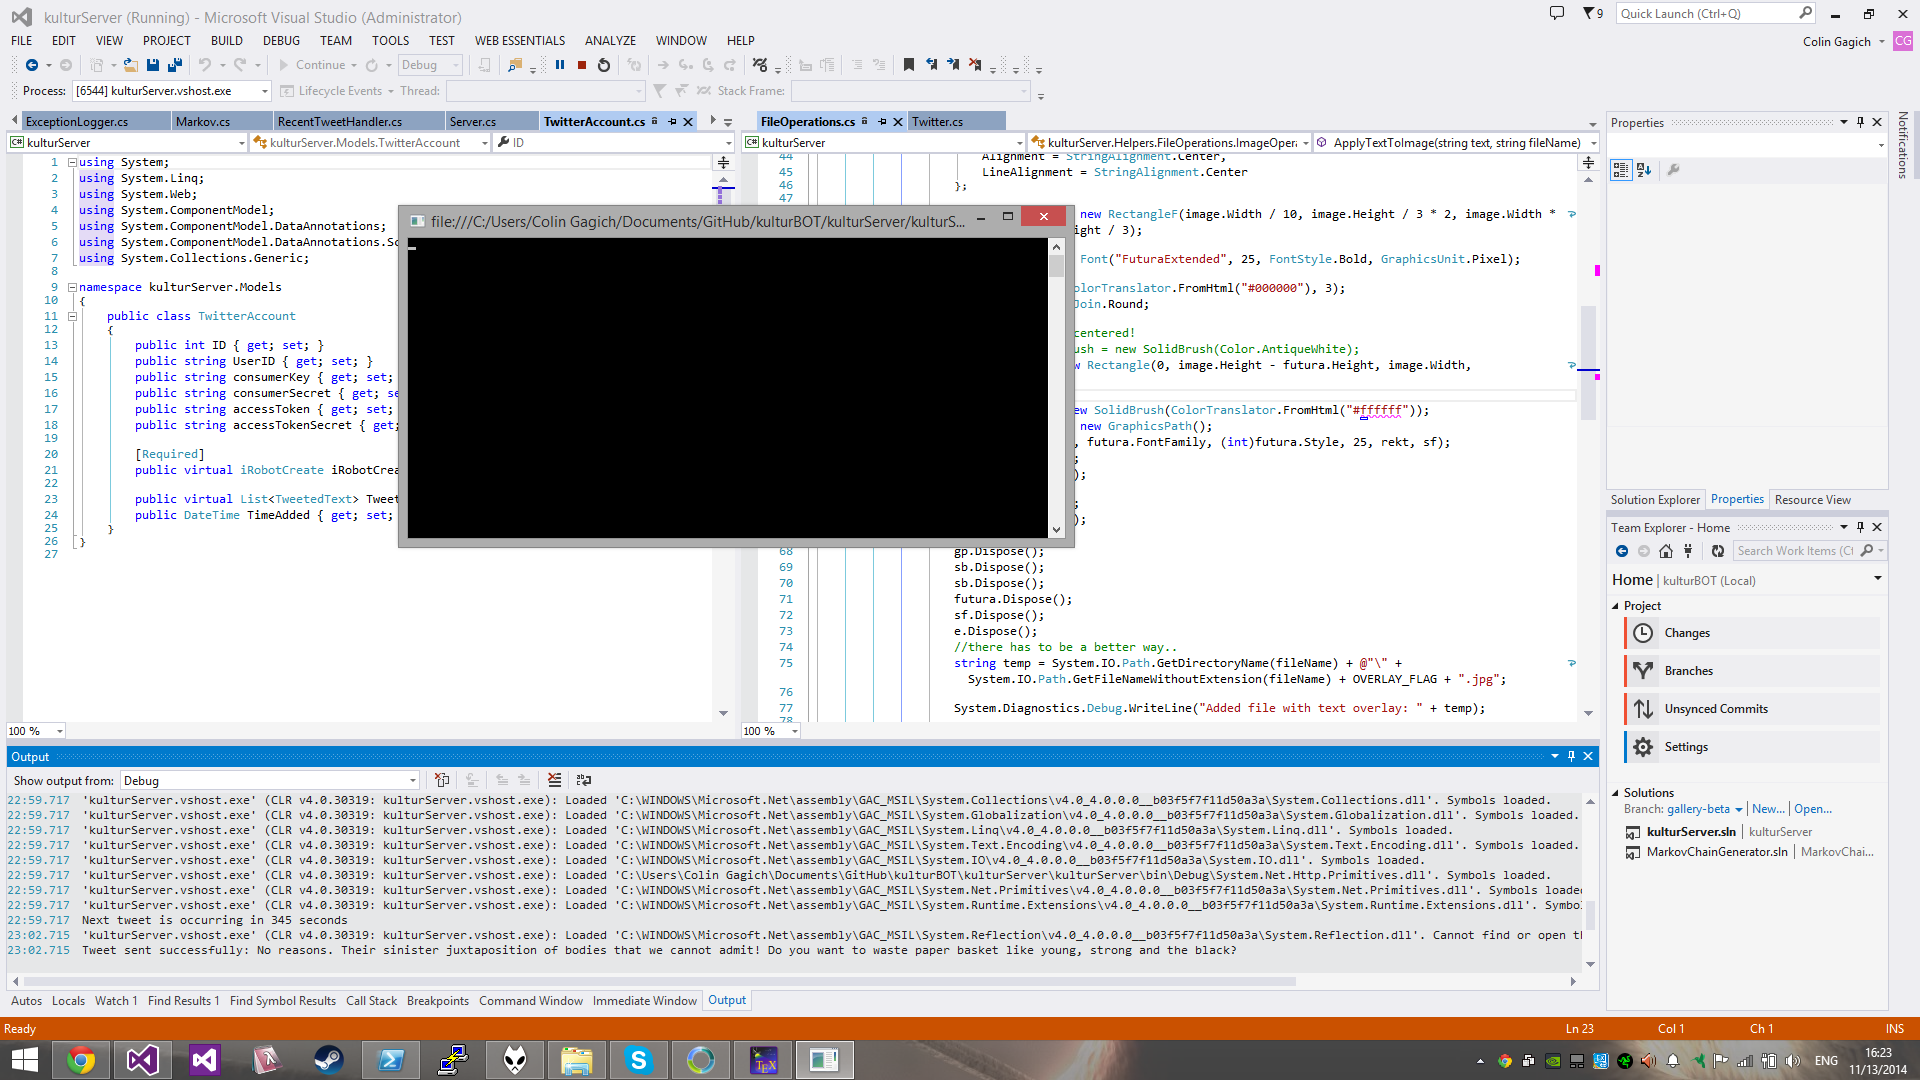
\includegraphics[width=1\textwidth]{img/normalVSlook.png}
	    \caption{Normal Operation of the Laptop}
	\end{figure}
	
	\item After you have done this, check the \href{https://twitter.com/kulturBOT}{\kbspace twitter feed} and ensure a tweet has been sent in the last 60 seconds.
\end{enumerate}
\begin{lstlisting}[frame=single]
THIS IS CODES
\end{lstlisting}

\section{Troubleshooting}
\subsection{\kbspace is taking pictures but not moving.}
\subsection{\kbspace won't turn on.}
\end{document}          
